\chapter{ZEEK}
As mentioned before the choosen tool for testing the data generated is ZEEK \cite{zeek}. This tool ha many functionalities
but the one that we used is the Network Intrusion Detection System.
ZEEK is not only that, in fact it is a passive, open-source network traffic analyzer. That means it supports
a wide range of traffic analysis tasks beyond the security domain, including performance measurement and 
troubleshooting. Many people use it as a Network Security Monitor or NSM, that is the collection and analysis
of security informations to discover presence of hints and facts about an intrusion in the network of a 
company.
\\\\
The usage of ZEEK aims to get an extensive set of logs, describing the network activity. These logs often 
includes a comprehensive record of every connection seen on the wire and an application-layer transcript. For
example theese can include HTTP session, with URIs and all sort of usefull information about the connections 
and the general browsing activity.
\\\\
By default, ZEEK uses a JSON log formatted file or a file well-structured and tab-separated: in that way the 
informations collected can easily be used for further analysis or post processing using external software.
A common way to store these data is in an external database or SIEM, so users can consume, store, process 
and present data for quering.
\\\\
In addition to the logs, ZEEK has build-in functionalities for a range of analysis and detection tasks, for
example: extractiong files from HTTP session, detecting malware using external registers, reporting 
vulnerabilities seen on the network, detecting bruteforce for SSH or validating SSL certificates.
\\\\
This tool is also a customizable and extensible platform for traffic analysis. In fact it provides the users 
a domain-specific, Turing-complete scripting language for expressing analysis tasks. The ZEEK language 
comes with a large set of pre-build functionalities, like a standard library, and users can write custome 
code. Indeed, all of defalult analyses, including logging, are done vie scripts; no specific analysis is 
hard-coded in the system.
\\\\
ZEEK can run also on low budget hardware and hence can be a low-cost alternative to expensive propetary 
solutions. In many ways this software exceeds the capabilities of other network monitoring tools, that 
remain limited to a small set of hard-coded tasks. ZEEK is not a signature-based Intrusion Detection 
System (IDS); while supporting this functionality, the scripting language facilitates a broader spectrum of 
different approaches to find malicious activities. These include semantic misuse detection, anamaly detection 
and behavioral analysis.
\\\\
This tool also support scalable load-balancing so it can be used for high-performance scenarios. Large site 
and organizations can use ZEEK Clusters, in which high-speed front end load balancer distributes the traffic 
across an appropiate number of back end PCs, running dedicated ZEEK instances on individual traffic slices.
\\
A Central Management System is used to coorinate the process, synchronizing state across the back ends and 
providing the operators with a central management interface for configuration and get aggregates logs. In that
way ZEEK can be used in both single and multi systems setups.
\\\\
In conclusion ZEEK is optimized for interpreting network traffic and generate logs, based on the traffic 
analyzed. It's not optimized for byte mathcing and users seeking signature detection approaches, like 
Intrusion Detection Systems do, and is not a protocol analyzer, seeking for depict every element of traffic 
at the frame level like Wireshark do. Zeek is in the middle seeking to get high fidelity network logs,
generating better understanding of network traffic and usage do. Zeek is in the middle seeking to get high 
fidelity network logs, generating better understanding of network traffic and usage.
\section{Architecture}
In this part we describe, at a very high leve, the ZEEK architecture. ZEEK is composed by various layers.
The \textit{event engine} (or core) reduces the incoming packet steam into a series of higher-level 
\textit{events}. These events reflect the network activity in policy-neutral terms, they describe what has 
been seen but not why or if it is important.
\\\\
For example, an HTTP request turns into an \textit{http$\_$request} event that carries the usefull informations,
like the IP addresses and ports, URI, HTTP versions and values. The event however does not convey any 
further interpretations, such as if the URI corresponds to a malware site.
\begin{figure}[h]
    \centering
    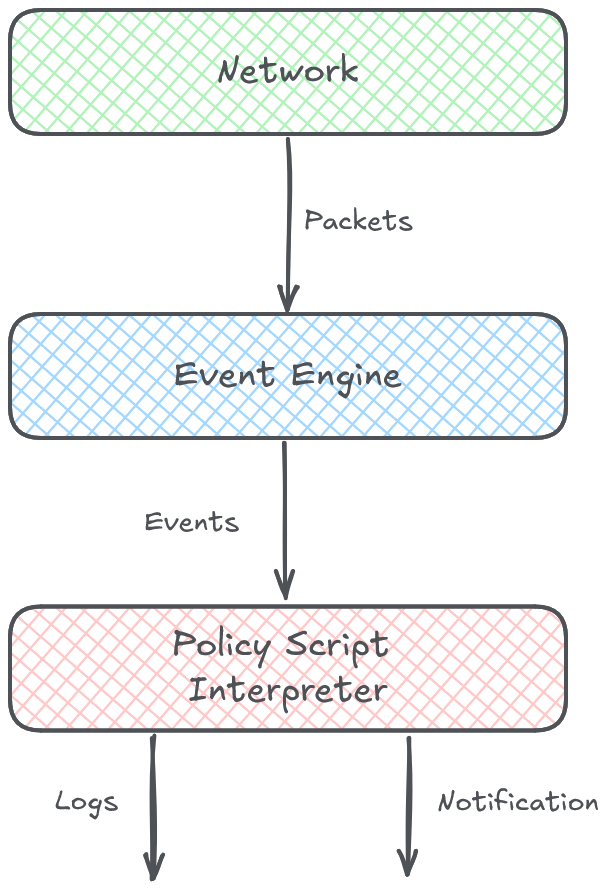
\includegraphics[width=4cm]{./architettura.png}
    \label{architecture}
    \caption{Architecture of ZEEK}
\end{figure}
$\\\\$
The event engine component comprises a number of subcomponents, including in particular the packet processing
pipeline consisting of: input sources, packet analysis, session analysis and file analysis. Input sources 
incest incoming network traffic from network interfaces. Packet analysis process lower-level protocols, 
starting all the way down at the link layer. Session analysis handles application-layer protocols, such as 
HTTP, FTP, and so on. File analysis dissects the content of files transferred over sessions. The event 
engine provides a plugin architecture for adding any of thes from outside of the core ZEEK code base, allowing
to expand ZEEK's capabilities as needed.
\\\\
Semantics related to the events are derived by the second main layer: the \textit{script interpreter}. This 
executes a set of \textit{event handlers} written in ZEEK language. These scripts can express a site's 
security policy, such as what actions to take when the monitor detects different types of activity.
\\\\
More generally scripts can derive any properties and statistics from the traffic. All ZEEK outputs 
comes from scripts included in the distribution. The language can generate real-time alerts and execute 
external programs on demand. One might use this functionality to trigger an active response for attack.
\\\\
With this we had introduced what ZEEK is and briefly how it works.
